\documentclass[conference]{IEEEtran}
\setlength{\parindent}{10pt}
%\IEEEoverridecommandlockouts
% The preceding line is only needed to identify funding in the first footnote. If that is unneeded, please comment it out.
\usepackage{cite}
\usepackage{amsmath,amssymb,amsfonts}
\usepackage{algorithmic}
\usepackage{graphicx}
\usepackage{textcomp}
\usepackage{listings}  % code
\usepackage{fancyvrb}
\usepackage{lipsum}
\usepackage{hyperref}
\usepackage{booktabs} % for excel
\usepackage{array} % for excel
\usepackage{multirow} % for excel
\usepackage{float} % solve pictures and sheets not follow by words issue! just like fucking Apple's Pages

\def\BibTeX{{\rm B\kern-.05em{\sc i\kern-.025em b}\kern-.08em
    T\kern-.1667em\lower.7ex\hbox{E}\kern-.125emX}}
\begin{document}

\title{Detecting and Preventing ARP Poisoning in SDN Networks}

\author{\IEEEauthorblockN{1\textsuperscript{st} Zhou, Yating}
	\IEEEauthorblockA{\textit{Department of Computer Science} \\
		\textit{Illinois Institute of Technology}\\
		Chicago, IL, USA \\
		yzhou115@hawk.iit.edu}
	\and
	\IEEEauthorblockN{2\textsuperscript{nd} Dugger, John}
	\IEEEauthorblockA{\textit{Department of Computer Science} \\
		\textit{Illinois Institute of Technology}\\
		Chicago, IL, USA \\
		jdugger@iit.edu}
	\and
	\IEEEauthorblockN{3\textsuperscript{rd} Sharma, Navjot}
	\IEEEauthorblockA{\textit{Department of Computer Science} \\
		\textit{Illinois Institute of Technology}\\
		Chicago, IL, USA \\
		nsharma11@hawk.iit.edu}
}

\maketitle


\begin{abstract}
This paper describes a method to detect and prevent Address Resolution Protocol (ARP) spoofing activities present in software-defined networks (SDN) by developing a POX controller application. The solution presented monitors for ARP poisoning activities by acting as a DHCP server and generating and maintaining an IP:MAC mapping in the controller and then routing all ARP and DHCP packets received by the switches to the controller with flow rules. It also provides countermeasures to address these malicious activities. We evaluate the performance by verifying consistency of host routing tables during and following an ARP attack, and we evaluate the additional load that an ARP attack places on the controller both with and without our defense in place. Throughout the paper, we refer to ARP Spoofing and ARP poisoning interchangeably.\\
\end{abstract}

\begin{IEEEkeywords}
Software-Defined Networks, SDN, Address Resolution Protocol, ARP, POX controller, Mininet, Amazon Web Services, AWS, ARP Poisoning, ARP Spoofing
\end{IEEEkeywords}

\section{PROBLEM STATEMENT}
Despite its many benefits, software-defined networks (SDNs) are still vulnerable to many malicious attacks such as spoofing, denial of service (DoS), tampering, repudiation, info disclosure, and elevation of privilege. If attackers compromise the network entities, it may lead to loss of sensitive information or even a shutdown of the entire network. Although well-defined solutions exist on most modern networks, many of the solutions rely on “smart” switches that contain both control and data plane elements to perform cryptographic validation. In an SDN, the switches no longer have the capacity to handle the mitigations since the control plane has been relocated to a centralized controller. This creates a unique opportunity to reinvent these tools as an application on top of the SDN controller. An SDN controller maintains a centralized view and control of the network which puts it in an ideal position to recognize and combat spoofing attacks.

\subsection{Address Resolution Protocol}
To understand our approach to ARP poisoning detection and prevention, it is important to fully understand the underlying protocol.

ARP is a critical component of any network since it allows any device on the local area network (LAN) to determine the physical (MAC) address of another device given only its logical (IP) address \cite{b10}. Operating in the data link layer, this protocol specifies both \texttt{ARP\_Request} and \texttt{ARP\_Reply} messages. If a device receives a packet and does not have a record of which physical device corresponds to the IP address contained in the packet, it broadcasts a \texttt{ARP\_Request} message to the other devices on the network. The \texttt{ARP\_Request} message contains the IP address the originator is attempting to resolve into a physical address. When a device receives an \texttt{ARP\_Request} message, it checks to see if it holds the IP address contained in the message. If it does, the receiving device transmits an \texttt{ARP\_Reply} message to the originator that associates its MAC address with the IP address.

Below is an example of a series of ARP messages where host 1 at 0:80:c8:f8:4a:51 (192.168.99.35) pings host 2 at 0:80:c8:f8:5c:73. In the linux example below, the \texttt{ARP\_Request} message is called \texttt{arp who-has}.

{
\tiny
\begin{verbatim}
1 0:80:c8:f8:4a:51 ff:ff:ff:ff:ff:ff 42: arp who-has 192.168.99.254 tell 192.168.99.35
2 0:80:c8:f8:5c:73 0:80:c8:f8:4a:51 60: arp reply 192.168.99.254 is-at 0:80:c8:f8:5c:73
3 0:80:c8:f8:4a:51 0:80:c8:f8:5c:73 98: 192.168.99.35 > 192.168.99.254: icmp: echo request (DF)
4 0:80:c8:f8:5c:73 0:80:c8:f8:4a:51 98: 192.168.99.254 > 192.168.99.35: icmp: echo reply
\end{verbatim}
}

One thing to notice is that, in the \texttt{ARP\_Reply} message, the originating MAC address matches the is-at reply. There should be no case where the is-at does not match the originating MAC address for the reply packet.

To prevent continually flooding the network with ARP messages, each device maintains a cached list of IP address - MAC address associations. Upon receiving a packet, a device first checks if the IP address contained in the packet is already on its ARP cache and only initiates an \texttt{ARP\_Request} if it is not cached. 

However, ARP is a stateless protocol, meaning that a device does not keep track of what physical addresses it has requested. Therefore, it is, by necessity, a trusting protocol that requires a device to update its ARP cache whenever an \texttt{ARP\_Reply} message is received, making it very vulnerable to cache poisoning.

Cache poisoning occurs when a malicious device or attacker sends an \texttt{ARP\_Reply} message that associates another device's IP address with the attackers MAC address. This results in packets that were intended for the other device to be instead routed to the attacker and is often used as an opening for other attacks such as denial of service, man in the middle, or session hijacking attacks.

\subsection{Software-Defined Networks}
The second concept to fully understand is the software-defined network. Software-Defined Networking is an emerging architecture that is dynamic, manageable, cost-effective, and adaptable, making it ideal for the high-bandwidth, dynamic nature of today's applications\cite{b11}. Most importantly, it moves the control logic out from each network device into a logically centralized controller. The controller then has a complete view of the network and can establish flow rules in each switch to control traffic flow in the network. This centralized visibility is the key feature that enables effective attack detection and prevention.

\subsection{Attack Vectors}
In order to be a successful product, our solution needs to be able to identify and protect against all forms of ARP poisoning attacks.
\begin{itemize}
    \item ARP Request packets are considered spoofed if any of the following are true
    \begin{itemize}
        \item Source MAC address of the ethernet header and source MAC address of the ARP header are not the same.
        \item Destination IP address in the ARP header is not present in th known hosts list of the DHCP server.
        \item The MAC address binding present in the known hosts list for the Source IP of the ARP header does not match with the source MAC address of the ARP header.
    \end{itemize}
    \item ARP Reply packets are considered spoof if any of the following are true
    \begin{itemize}
        \item Source MAC address of the ethernet header and source MAC address of the ARP header are not the same.
        \item Destination MAC address of ethernet header and destination MAC address of ARP header are not the same.
        \item The MAC address binding present in the known hosts list for the Source IP of the ARP header doesn't match with the Source MAC address of the ARP header
        \item The MAC address binding present in the known hosts list, for the Destination IP of the ARP header doesn't match with the Destination MAC address of the ARP header
        \item Destination MAC address of the ethernet header has a value of FF:FF:FF:FF:FF:FF.
    \end{itemize}
\end{itemize}
 
\section{PRIOR WORK}
Previous work to combat ARP poisoning includes SPHINX\cite{b1} which uses the metadata when a \texttt{PACKET\_IN} arrives to build a flow graph that maintains and updates MAC-IP bindings for all hosts in the network along with a list of possible switch-ports at which they can be located. However, upon detective a deviation, it merely raises an alert. Our approach, built as an application instead of a proxy, can direct flow rules to correct any deviations discovered.

Our approach is heavily based on Cisco's Dynamic ARP Inspection (DAI)\cite{b12} which is proprietary software included on Cisco switches. It is implemented on "smart" switches (i.e., not SDN switches) and builds a database of trusted bindings based on snooping DHCP packets. It then requires that the switch intercepts, logs, and discards ARP packets with invalid IP-to-MAC address bindings that do not appear in its database of trusted bindings. Since the switches in an SDN are separate from the control plane, DAI cannot be directly implemented. Additionally, the Cisco switches can only snoop DHCP packets that pass through them, so their view of the network is extremely limited. This results in false positives that are logged and need to be reviewed by an administrator. Additionally, it fails to protect against a rogue DHCP server from serving clients. As you will see below, our implementation within an SDN overcomes all of these shortcomings.

There have also been active techniques developed to detect ARP spoofing\cite{b13}. Active techniques are an excellent method of mitigating some of the shortcomings of the passive approach used in DAI. However, active approaches are unnecessary in an SDN where the controller both has a centralized view of the network and can act as the DHCP server.

There are also many programs available such as Arpwatch that need to be installed on every legitimate device in the network to effectively combat ARP poisoning. This approach works well in tightly controlled networks; however, it prevents users from being able to bring their own devices to the network without needing first to get the third party software installed which greatly limits its usability.

\section{RESEARCH APPROACH}
To design and build an application that is able to combat ARP poisoning, we built an environment using established tools, such as POX Controller, Mininet, OpenFlow protocol and an Amazon Web Services (AWS) platform.

Working with a distributed team is always a challenge. To effectively collaborate, we first needed to set up our network environment. For better cooperation, we deploying our network simulation environment (Ubuntu operating system) on AWS. For simulating arbitrary network topology, we installed mininet on AWS. For communication protocol between network switches and network controller, we used OpenFlow to forward the packet to the controller, which is a communications protocol that gives access to the forwarding plane of a network switch or router over the network. The controller we are using is a POX controller upon which we wrote the ARP detection and prevention application.

Figure \ref{fig:SDN}, shows an architectural view of SDN network setup using POX Controller, and the interaction between different components.

\begin{figure}[ht!]
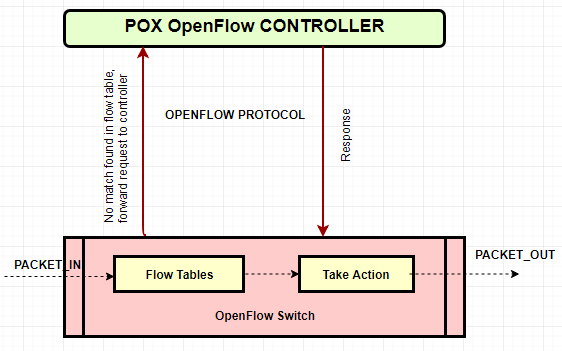
\includegraphics[width=0.5\textwidth]{Figure_1.png}
\caption{Architectural view of SDN}
\label{fig:SDN}
\end{figure}


\subsection{POX Controller}
POX controller is an open source development platform which is used for developing Python based Software Defined Network (SDN) control applications. It is inherited from NOX, and enable rapid development and prototyping\cite{b8}.

Building on the POX controller, we drew heavily upon the included dhcpd.py and l2\_learning.py. By starting from the level 2 learning switch included in the POX source code, we were able to directly implement our solution without needing to develop the basic switch structure\cite{b9}. POX also has a significant amount of community support and tutorials available since it has been around since 2011\cite{b3}.

%s our\cbeeg in{figure}[H]
% 	\centerline{\includegraphics[scale=0.4]{intro1-2.png}}
% 	\caption{The software product line engineering framework}
% 	\label{fig}
% \end{figure}

\subsection{Mininet Network Topology}
Mininet is a network emulator, or perhaps more precisely a network emulation orchestration system\cite{b2}. It runs a collection of end-hosts, switches, routers, and links on a single Linux kernel. It uses lightweight virtualization to make a single system look like a complete network, running the same kernel, system, and user code. A Mininet host behaves just like a real machine; you can ssh into it (if you start up sshd and bridge the network to your host) and run arbitrary programs (including anything that is installed on the underlying Linux system.). We have implemented a custom topology with one controller, one switch and three hosts.

Figure \ref{fig:topology} show the mininet custom topology that we created for setting up our SDN network.

\begin{figure}[ht!]
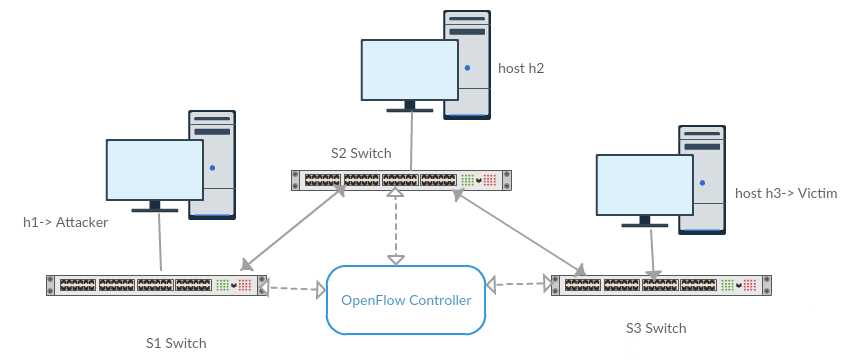
\includegraphics[width=0.5\textwidth]{figure4.png}
\caption{Mininet customized topology}
\label{fig:topology}
\end{figure}



\subsection{OpenFlow protocol}
OpenFlow is a protocol that allows a server to tell network switches where to send packets. In a conventional network, each switch has proprietary software that tells it what to do. With OpenFlow, the packet-moving decisions are centralized, so that the network can be programmed independently of the individual switches and data center gear. In a conventional switch, packet forwarding (the data path) and high-level routing (the control path) occur on the same device. An OpenFlow switch separates the data path from the control path. The data path portion resides on the switch itself; a separate controller makes high-level routing decisions. The switch and controller communicate by means of the OpenFlow protocol. This methodology, known as software-defined networking (SDN), allows for more effective use of network resources than is possible with traditional networks.

\subsection{AWS}
We used Amazon Web Services (AWS) to create the environment for this project. AWS is a secure cloud services platform, offering computing power, database storage, content delivery and other functionality to help businesses scale and grow.

\section{IMPLEMENTATION, USAGE AND ANALYSIS}
The implementation will follow the same order as how we implement or coding all the stuff. Since we did not have useful ARP spoofing attack tools at hand, we have to write our own spoofing attack utility first. Once we finish the attack tools, we can then implement our own controller. In additional, scripts largely increase our productivity during testing. 

\subsection{ARPSpoof}
\textbf{ARPSpoof} is a tool set providing users the ability to perform a real ARP spoofing attack on a given network topology. The reason to why we use C++ is because it generally provide us some essential benefits in our experiment: 
\begin{itemize}
\item Reduce the context switching so that it will not affect the pox performance under minet
\item Mdularize due to Object-Orient Programming so that the main logic in the attack tool sets is easy for user to understand 
\item Cross platform, it can be executed without too much dependencies on any platforms (Windows, GNU/Linux or even macOS)
\item Easy to use
\item High efficiency so that it can deploy on both AWS, Virtualbox or even Raspberry Pi without punishment
\end{itemize}
With this in mind, the general logic of how we designed the ARPSpoof is as following:
\begin{itemize}
    \item Get arguments from user (e.g. router IP, victim IP)
    \item Initialize FakeARPPacket with router IP and viticm IP
    \item Set victim MAC address and router MAC address
    \item Get and set interface from current host interface
    \item Send fake arp (request vs. reply) packets to victim host
\end{itemize}
The source code is available here. To use it, just simply jump right into the source folder, then type in '\textbf{make}', it will then generate two executable binaries: request and reply. In addition, the arguments of these two attack programs are as following:

{
    \tiny
    \begin{verbatim}
    request [router IP] [victim IP] [replay]
    request [interface] [router IP] [victim IP] [replay]
    reply [router IP] [victim IP] [replay]
    reply [interface] [router IP] [victim IP] [replay]
    \end{verbatim}
}

Note, '\textbf{replay}' is the number of arp packets we want to send out, negative replay indicates flooding out arp packets infinity. The '\textbf{interface}' argument will tell the FakeARPPacket object to set up the interface member from user instead of detecting by itself.

\subsection{SDNController}
There are several important routines worth mentioning: is \textit{msglog}(), \textit{\_handle\_PacketIn}(), \textit{arpPktShim}(), \textit{isARPInvalid}() and \textit{blockMAC}(). \textit{msglog}() provides an unparalleled beautiful output style of our controller, it tells user exactly all information from one event: the time, the status/result, and what event it is. All packets will be handled by calling \textit{\_handle\_PacketIn}(). In \textit{\_handle\_PacketIn}(), \textit{arpPktShim}() will get invoked if the packet type is ARP.  \textit{arpPktShim}() will check the arp packets through \textit{isARPInvalid}(), and call \textit{blockMAC}() if the arp is invalid arp packets. \textit{blockMAC}() blacklist the similar packets and source MAC for a while. In this case, intensive arp spoofing attack will not degrade the performance of our controller.

And all the members and functions are listed as Table. 1
\begin{table}[H]
		\caption{\textbf{FakeARPPacket} members table}
		\label{Tab:FakeARPPacket}
		\centering
		\begin{tabular}{lp{2cm}p{3cm}p{0cm}}
			\toprule
			\textbf{Member} &\textbf{Type} &\textbf{Function}&\\
			\midrule
			interfaceNo        &int  	&interface number    \\\\
			routerIP           &char*  & fake router IP\\\\
			victimIP           &char*  & victim IP \\\\   
			routerMAC          &uint8\_t[] & fake rounter MAC address\\\\
			victimMAC          &uint8\_t[] & victim MAC address \\\\
			\midrule
			\textit{FakeARPPacket}()    & constructor\&\& & constructors \\\\
			\textit{sendRequestPkt}()    & void(*)      & send request arp packet\\\\
			\textit{sendReplyPkt}()      & void(*)      & send reply arp packet\\\\
			\textit{getInterfaceNo}()    & int(*)       & get interface number\\\\
			\textit{getRouterIP}()       & char(**)       & get router IP address\\\\
			\textit{getVictimIP}()       & char(**)     & get victim IP address\\\\
			textit{getRouterMAC}()       & uint8\_t(*[]) & get router MAC address\\\\
			textit{getVictimMAC}()       & uint8\_t(*[]) & get victim MAC address\\\\ 
			\textit{setInterfaceNo}()    & void(*)       & set interface number\\\\
			\textit{setRouterMAC}()      & void(*)       & set router MAC address\\\\
			\textit{setVictimMAC}()      & void(*)       & set victim MAC address\\\\
			\textit{setRouterIP}()       & void(*)       & set router IP address\\\\
			\textit{setVictimIP}()       & void(*)       & set victim IP address\\\\
			\bottomrule
		\end{tabular}
\end{table}


\subsection{Launch scripts}
As we know, implementation and running through all the steps like starting the controller, initializing the network topology and performing all the test cases are not as trivial as we though, there's large amount of commands need to be typed in one-by-one. If mistakes happens while testing, we need to re do/type all the commands by hand, which is tedious and not efficient. To solve this problem in order to provide both flexibility and high efficiency while debugging. All the handy scripts and its usage can be seen in Table. 2
\begin{table}[H]
		\caption{\textbf{Misc} programs table}
		\label{Tab:Scripts}
		\centering
		\begin{tabular}{lp{3cm}p{2cm}p{0cm}}
			\toprule
			\textbf{Name} &\textbf{Function}&\\
			\midrule
			initController        &initialize SDNController   \\\\
			initNet               &initialize mininet topology\\\\
			dhcp                  &get current ethernet interface and DHCP current host\\\\
			push                  &push changes to upstream\\\\
			\midrule
			request               &send fake arp request packets\\\\
			reply                 &send fake arp reply packets\\\\
			\bottomrule
		\end{tabular}
\end{table}

Since we need to protect against ARP Spoofing Attacks on controller (or switches) at l2 level, so that one of the most important steps is to simulate the ARP Spoofing attacks within the network we just created. Once we implemented the ARP Spoofing attacks in SDN, we then can try to track the log from the controller or switches and try to mitigate the issue in our SDNController program. We have successfully implemented the ARP spoofing attacks in our network topology, without losing the generality, suppose the following network topology: one controller (c0), three switch (s1, s2, s3), three hosts (h1, h2, h3 respectively) that are attached as follows: (h1, s1), (h2, s2), (h3, s3), (s2, s1), (s3, s2)\newline

The h3 is the victim, and the h1 is the ARP spoofing attacker 
Now we can execute the attack from h1 then check against each of the ARP table on each of the host to see if the table has been infected. \newline

By using the mininet, we gradually know how to use mininet to initialize the network topology we want. By using the ARP spoofing attack and look into the source code, we learned more about what exactly ARP spoofing is doing, which leads us to generalize the ARP spoofing in our simulation network later on. We in order to implement the enhanced POX based controller and an enhanced switches to protect against the ARP spoofing attacks and figure out the fix up the ARP cache poisoner for each of the host, our basic rules are as follows:\newline
TO DETECT ARP SPOOFING:\newline
Generating and maintaining routing table in controller.\newline
Routing ARP and DHCP packets to the controller with flow rules.\newline
Detecting ARP attack if any of the following cases are false:
\begin{itemize}
\item Check if the packet’s ethernet src MAC == ARP src MAC
\item Check if the ARP packet src MAC and ARP src IP are matched from the table
\item Check if the ARP destination IP exists in the table
\end{itemize}
Detecting ARP attack if any of the following cases are true:
\begin{itemize}
\item ARP replies with no ARP requests
\item Multiple ARP replies with only one ARP request
\end{itemize}
TO MITIGATE ARP SPOOFING:
\begin{itemize}
\item Do not allow ARP packets identified as attack packets to be forwarded
\item Generate Flow rule to drop all packets coming into switch on attacker’s port.
\end{itemize}

An ARP packet identified will have below attributes as show in Figure \ref{fig:ARPPacket}.

\begin{figure}[h!]
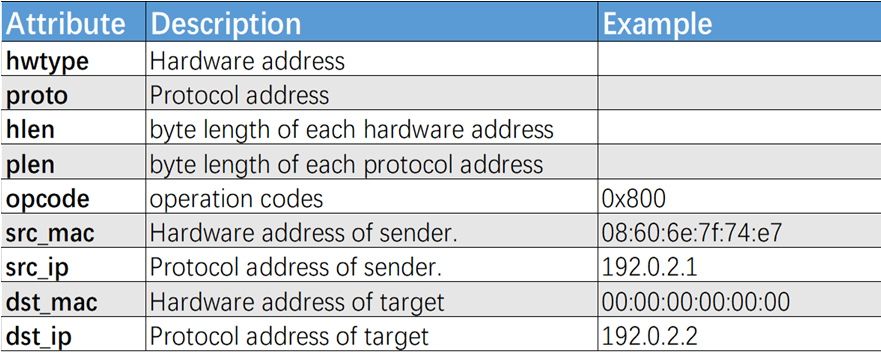
\includegraphics[width=0.5\textwidth]{Figure_2.png}
\caption{An ARP packet instance}
\label{fig:ARPPacket}
\end{figure}


Keeping above implementation in mind, we have come up with below flow chart in Figure \ref{fig:flowchart}, which explains the logic of detecting and mitigating ARP spoof attacks.

\begin{figure}[h!]
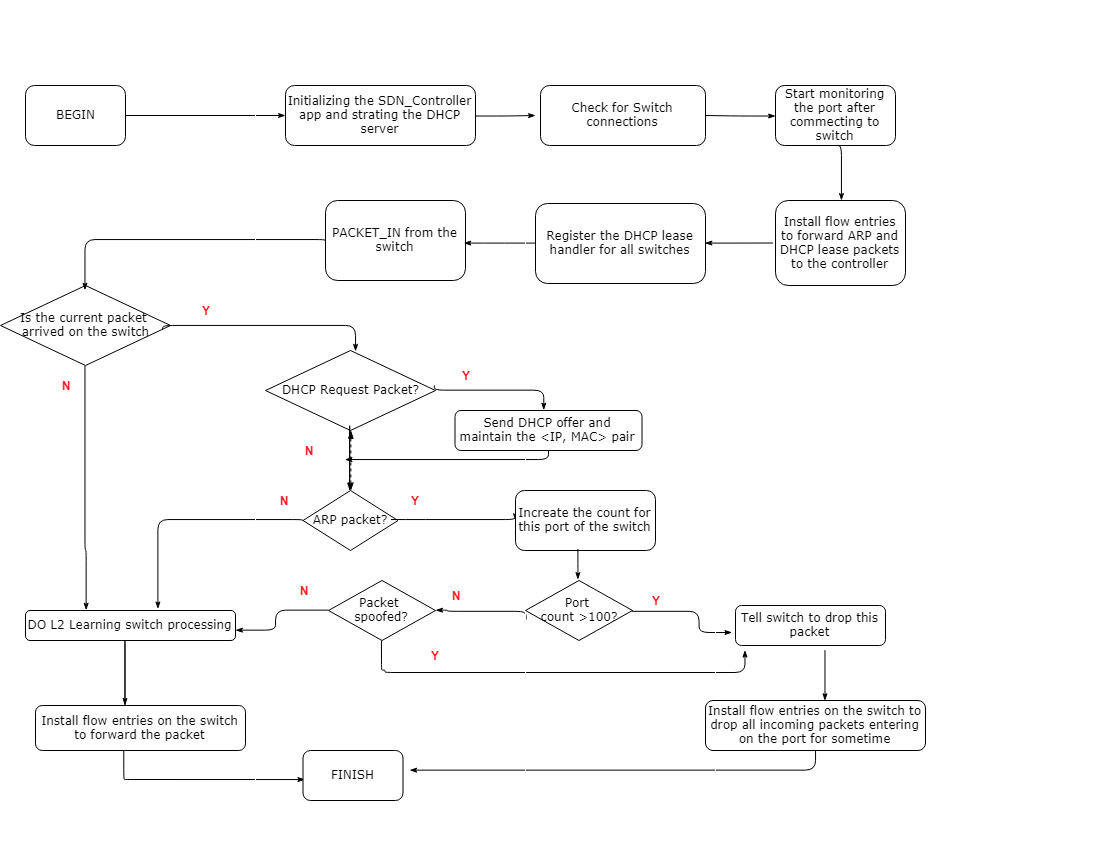
\includegraphics[width=0.5\textwidth]{figure3.png}
\caption{Flow Chart to detect and mitigate ARP spoof attack}
\label{fig:flowchart}
\end{figure}

Below figures from 5 to 9 shows the output screenshots of the experiment performed step by step:

\begin{figure}[h!]
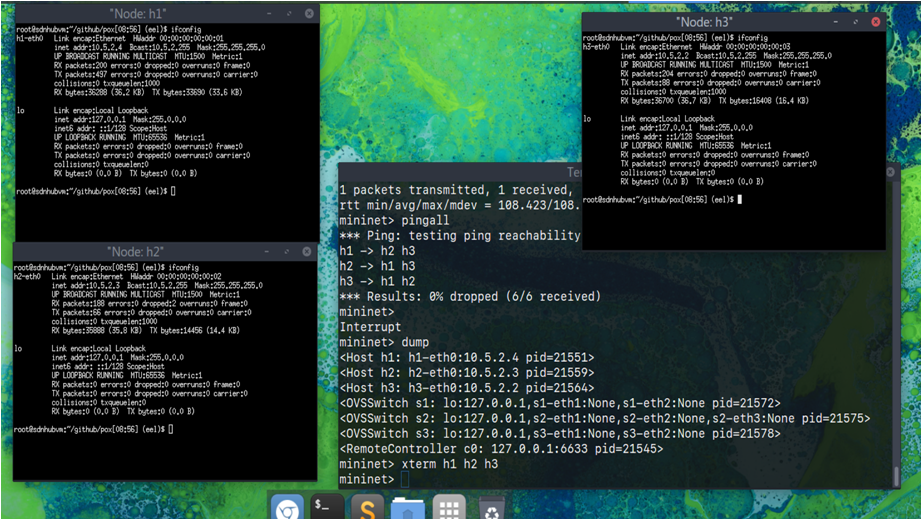
\includegraphics[width=0.5\textwidth]{out1.png}
\caption{Step 1}
\end{figure}

\begin{figure}[h!]
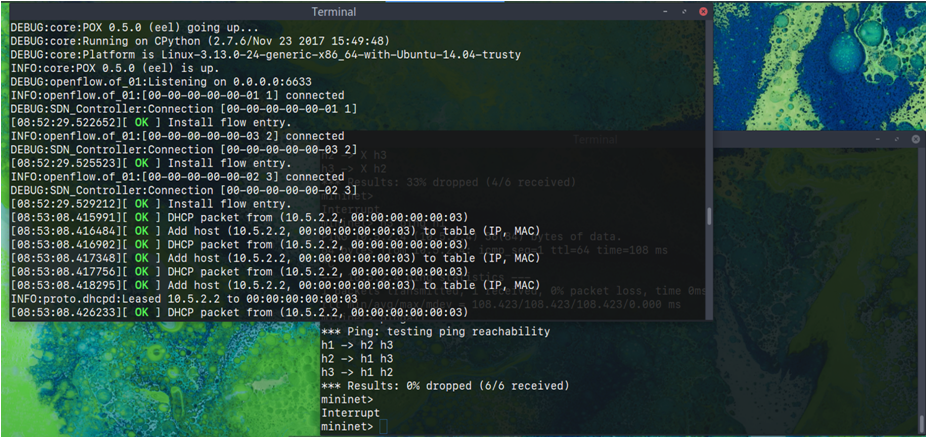
\includegraphics[width=0.5\textwidth]{out2.png}
\caption{Step 2}
\end{figure}

\begin{figure}[h!]
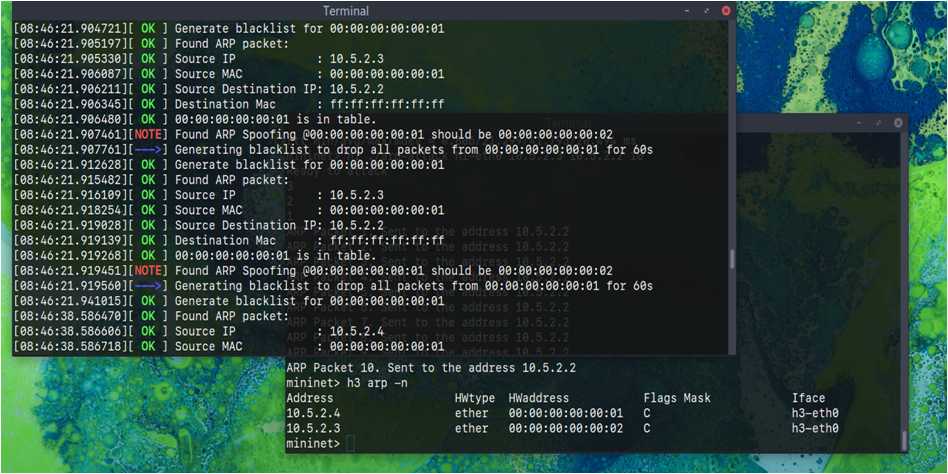
\includegraphics[width=0.5\textwidth]{out3.png}
\caption{Step 3}
\end{figure}

\begin{figure}[h!]
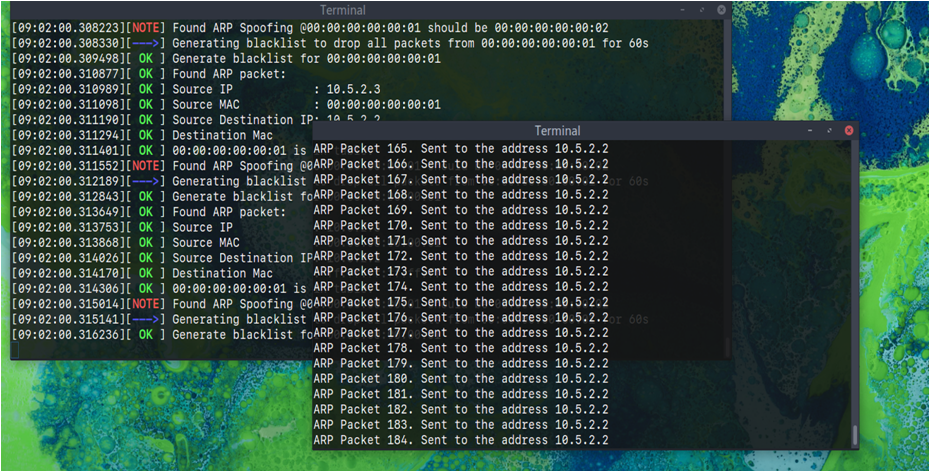
\includegraphics[width=0.5\textwidth]{out4.png}
\caption{Step 4}
\end{figure}

\begin{figure}[h!]
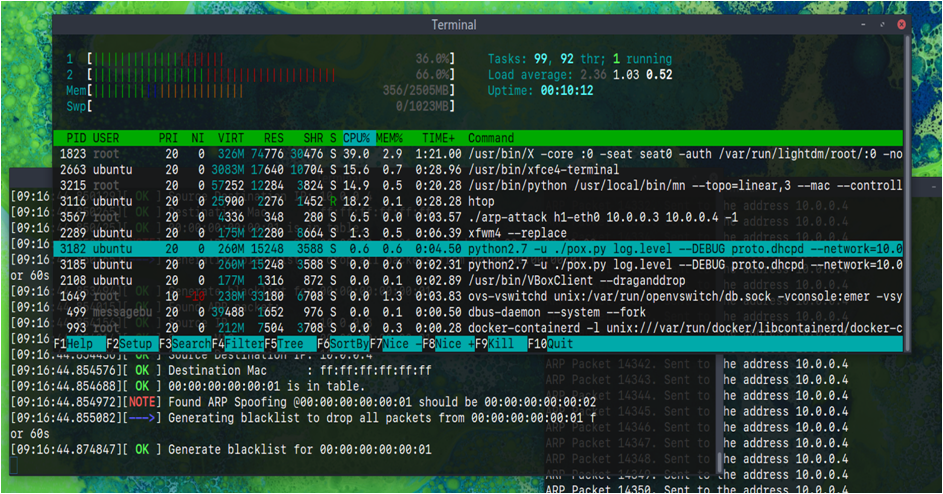
\includegraphics[width=0.5\textwidth]{out5.png}
\caption{Step 5}
\end{figure}


\section{PERFORMANCE EVALUATION}
When considering performance under a large scale in real world, protecting against ARP spoofing will not be an easy job since attackers will very likely flooding out intensive dummy ARP packets. Without carefully design of the controller will very easily use up all the CPU resources and memory resources handling even a simply forwarding. So that we must change our strategy and optimize our controller in order to maintain both protecting functionalists and forwarding functionalists. By analyzing the pattern of ARP attacking, we found out that ARP attackers will very likely flooding out intensive dummy ARP packets at a given period of time, in order words, we don't need to block all the dummy ARP packets at once, what we need to do is to simply block all the attack's ARP packets at a given period of time (e.g. 60 seconds, 120 seconds and etc.). By blocking the attackers for a given period of time, SDN Controller can free from busy blocking each of the dummy packets and thus maintaining both of the functionalists. Let's analyze the performance of our controller now.\\

\subsection{Softwares and techniques}
\begin{itemize}
    \item CPU: Intel(R) Core i7-4712 HQ @2.30 GHz with two cores available
    \item PAE/NX - Enabled
    \item Memory: 2560MB LPDDR3 @1600MHz Dual Channel
    \item Vitualization (Intel VT-x) - Enabled
    \item Ethernet bandwith: 1000Gb/s
    \item For previous coding - C, C++, Python and bash
    \item Operating Systems: Ubuntu 14.04.5 LTS
    \item For all configurations and environment setup - Bash
\end{itemize}

The command for the ARP spoofing will be the following:
{
\tiny
\begin{verbatim} 
h1 ./request \${fakeIP} \${targetIP} -1  
\end{verbatim}
}

\subsection{CPU Utilization Rate Analysis}

We monitored the resources usage rate from 1 second to 30 second, and we performed the attack at the 5\textsuperscript{th} second, and discarded the flooding attack at the 25\textsuperscript{th} second. The CPU utilization performance and their comparison are as Figure \ref{fig:CPUwProtection}, Figure \ref{fig:CPUwoProtection} and Figure \ref{fig:CPUComparison}.

\begin{figure}[h!]
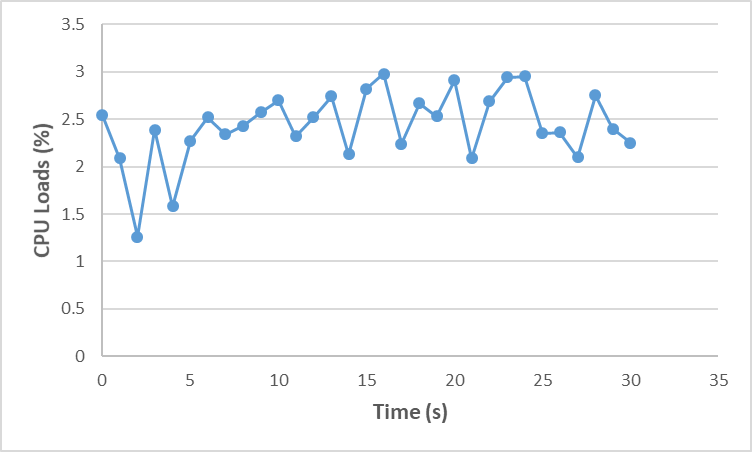
\includegraphics[width=0.5\textwidth]{CPUwProtection.png}
\caption{CPU utilization with protection}
\label{fig:CPUwProtection}
\end{figure}

\begin{figure}[h!]
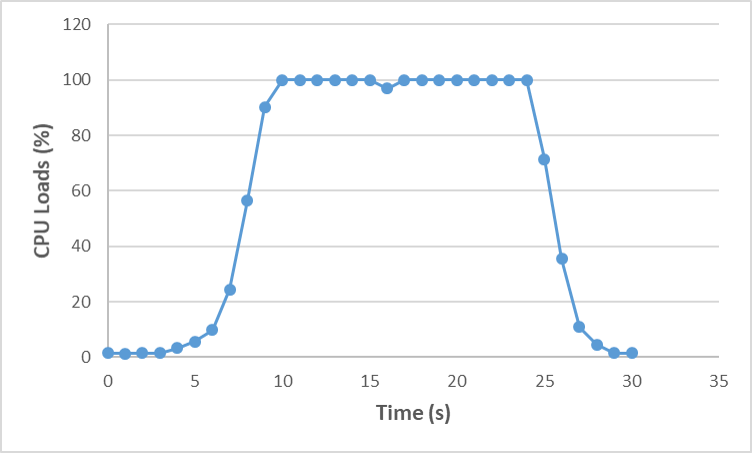
\includegraphics[width=0.5\textwidth]{CPUwoProtection.png}
\caption{CPU utilization without protection}
\label{fig:CPUwoProtection}
\end{figure}

\begin{figure}[h!]
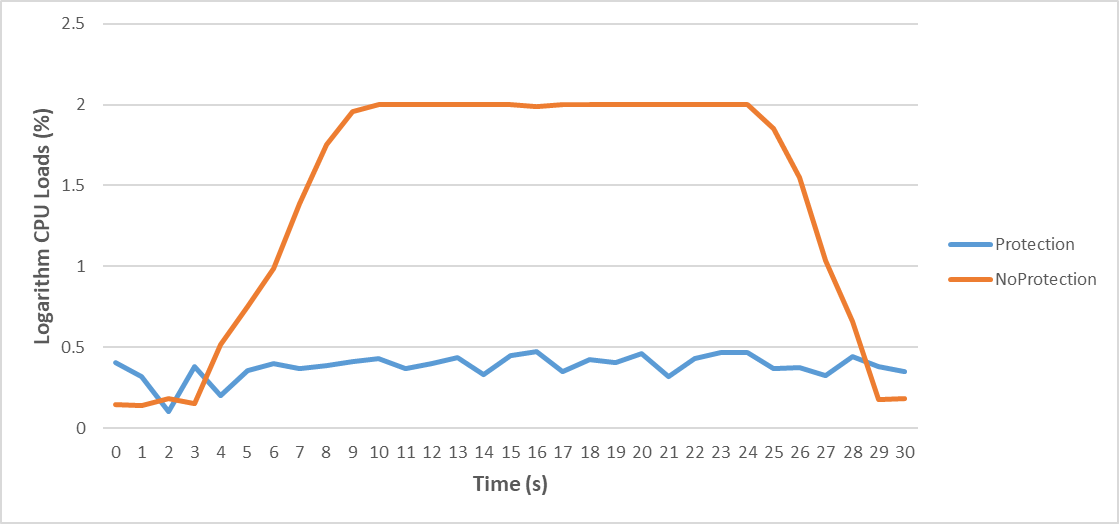
\includegraphics[width=0.5\textwidth]{CPUCompareLog.png}
\caption{CPU utilization rate (logarithm based 10) comparison}
\label{fig:CPUComparison}
\end{figure}

As we can see in the Figure \ref{fig:CPUwProtection}, Figure \ref{fig:CPUwoProtection} and Figure \ref{fig:CPUComparison}, before we initialize the attack (0s-5s), the CPU utilization rate of our SDN Controller is a bit higher than l2\_learning controller which is the default controller. The reason is because SDN Controller will check each of the ARP packets and DHCP packets, so it is as expected. When we executed the attack on each of the controller at 5\textsuperscript{th} second, the CPU utilization rate of l2\_learning controller is way higher than SDN Controller, this is because the default controller use up all the CPU resources while the utilization rate of SDN Controller almost remains the same thanks to the blacklist mechanism we discussed in previous section. Since the utilization rate of the default controller is way higher than our own controller, we took the logarithm with based 10 to compare both of the controllers as professor Kevin Jin's suggestion.

Since the controller's performance will also be affected by the performance of CPUs, so that we want to get rid of this kind of affect as well. In other words, if the CPU performance is excellent, the CPU utilization rate of any controller will be at a relatively low level, while a poor performance CPU will in the opposite high level. So this leads us to a more complete analysis using margin CPU utilization rate, which is calculated as the following formula:
\begin{align}
    M(t) = \frac{dU(t)}{dt}=M^{'}(t)
\end{align}
Here, $M(t)$ $U(t)$ is the CPU utilization rate at given time $t$, $M(t)$ is the margin CPU utilization rate. Higher the margin rate indicates the controller behave petty poor at the given period of time. What we expect is the CPU utilization rate remains in a very stable low level. The CPU margin effect and its comparison are as Figure \ref{fig:MCPUwProtect}, Figure \ref{fig:MCPUwoProtect} and Figure \ref{fig:MCPUComparison}.

\begin{figure}[h!]
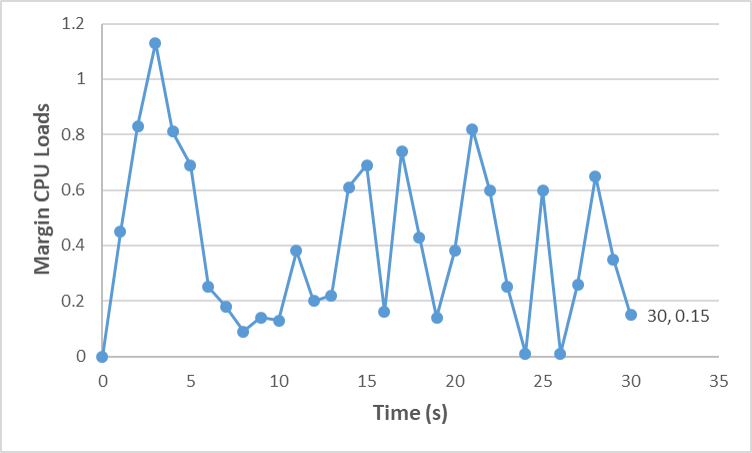
\includegraphics[width=0.5\textwidth]{MCPUwProtect.png}
\caption{CPU margin utilization rate with protection }
\label{fig:MCPUwProtect}
\end{figure}

\begin{figure}[h!]
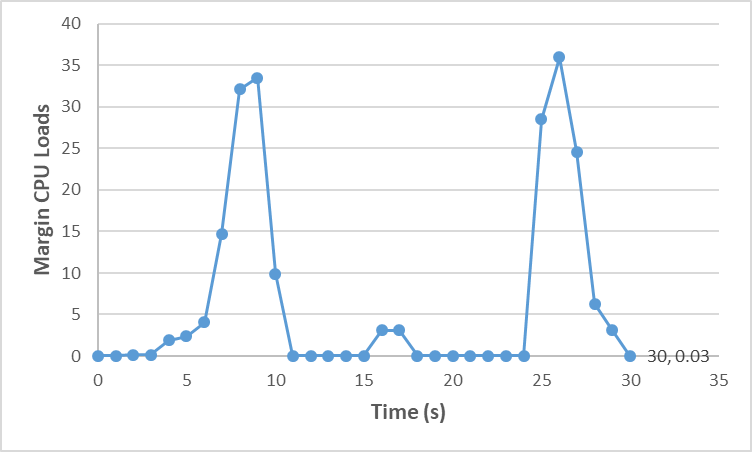
\includegraphics[width=0.5\textwidth]{MCPUwoProtect.png}
\caption{CPU margin utilization rate without protection}
\label{fig:MCPUwoProtect}
\end{figure}

\begin{figure}[h!]
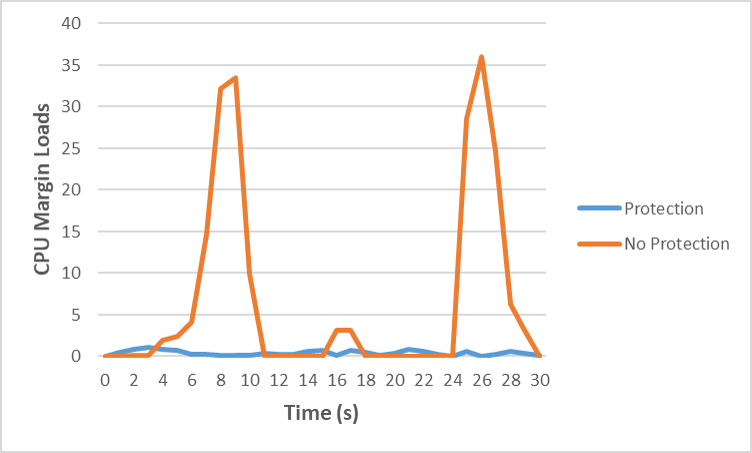
\includegraphics[width=0.5\textwidth]{MCPUComparison.png}
\caption{CPU margin utilization rate comparison}
\label{fig:MCPUComparison}
\end{figure}

As we can see that the around 5s - 10s the margin CPU rate of the default controller down to $0$, this indicates the fact that the default controller used up all the CPU resources, so that 
\begin{align}
     M(t) = \frac{dU(t)}{dt}=\frac{100-100}{dt}=\frac{0}{dt}=0
\end{align}
However, our SDNController behave pretty well and the CPU margin effect is almost invisible comparing to the default l2\_learning controller, in other words, SDNController even behaved stable under high volume of arp spoofing attacks. 

\subsection{Memory utilization rate analysis}
When we comes to analysis the memory utilization rate, we will then see some very interesting fact comparing to the CPU utilization rate analysis as Figure \ref{fig:MemwProtect}, Figure \ref{fig:MemwoProtect} and Figure \ref{fig:MemComparison}.

\begin{figure}[h!]
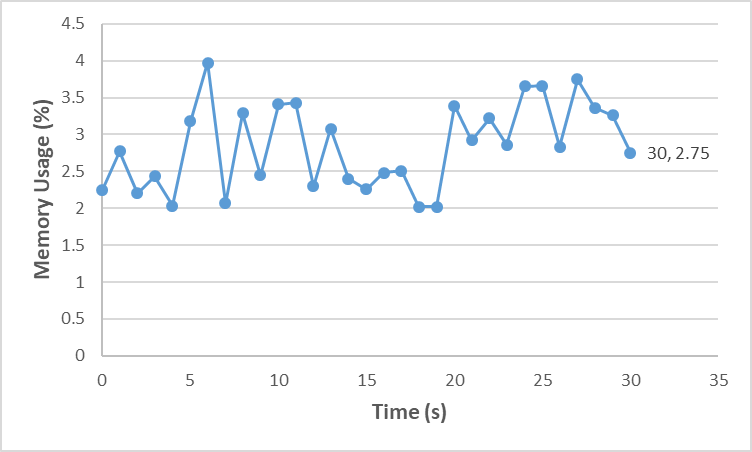
\includegraphics[width=0.5\textwidth]{MemwProtect.png}
\caption{Memory usage rate with protection}
\label{fig:MemwProtect}
\end{figure}

\begin{figure}[h!]
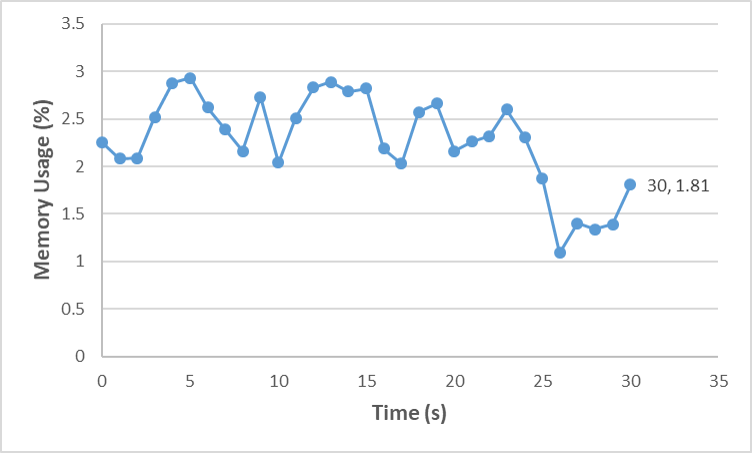
\includegraphics[width=0.5\textwidth]{MemwoProtect.png}
\caption{Memory usage rate without protection}
\label{fig:MemwoProtect}
\end{figure}

\begin{figure}[h!]
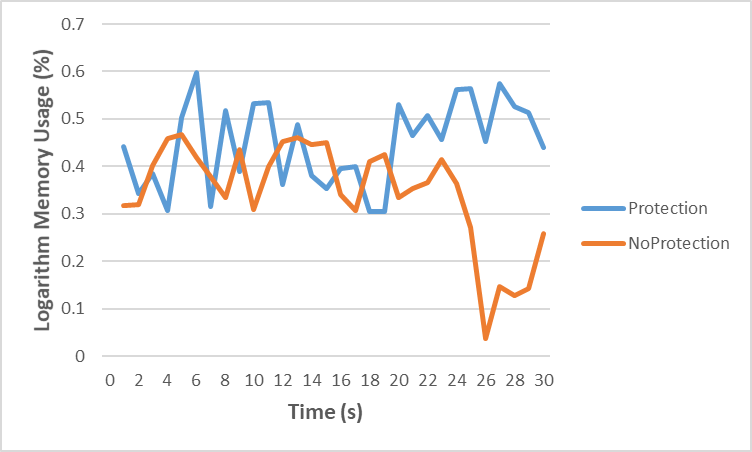
\includegraphics[width=0.5\textwidth]{MemComparison.png}
\caption{Memory usage rate (logarithm based 10) comparison}
\label{fig:MemComparison}
\end{figure}

As we can see in the Figure \ref{fig:MemwProtect}, Figure \ref{fig:MemwoProtect} and Figure \ref{fig:MemComparison}. The memory usage rate of the default controller is a bit lower than our SDNController, and the reason is because our controller has to maintain a $(IP, MAC)$ hash table so that it can protect against arp spoofing effectively. 

\subsection{Marginal effect of memory usage rate}
Similar to marginal effect of CPU utilization rate, the marginal memory utilization rate will be the following:
\begin{align}
    MemM(t) = \frac{dMemM(t)}{dt}=MemM^{'}(t)
\end{align}

It indicates the stability in memory while we launch the controller. 

\begin{figure}[h!]
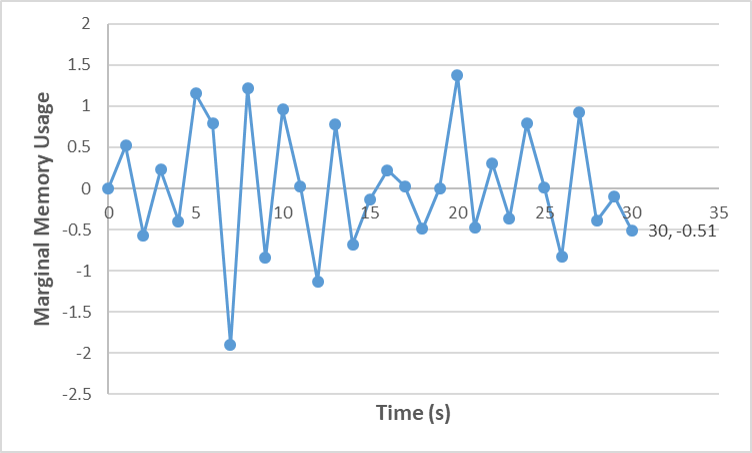
\includegraphics[width=0.5\textwidth]{MarginalMemwProtect.png}
\caption{Marginal Memory usage rate with protection}
\label{fig:MarginalMemwProtect}
\end{figure}

\begin{figure}[h!]
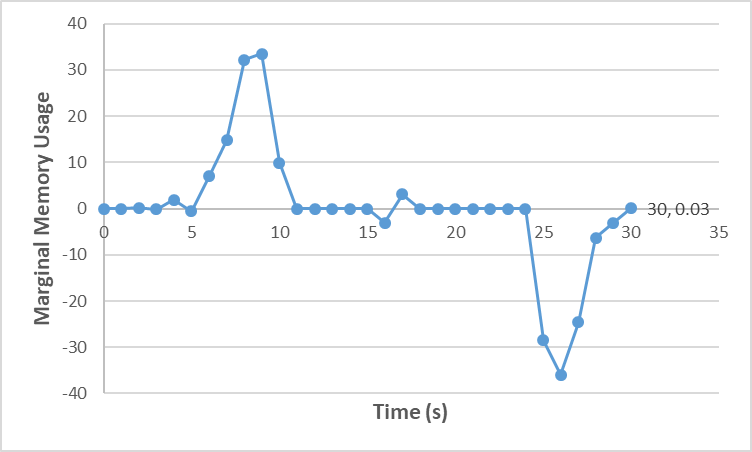
\includegraphics[width=0.5\textwidth]{MarginalMemwoProtect.png}
\caption{Marginal Memory usage rate without protection}
\label{fig:MarginalMemwoProtect}
\end{figure}

\begin{figure}[h!]
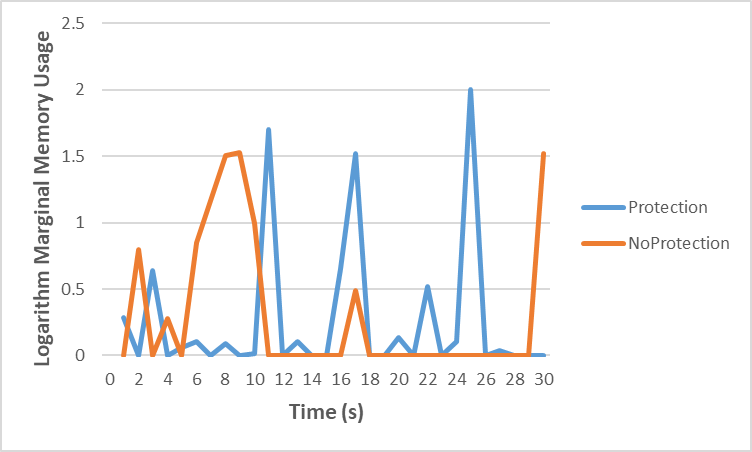
\includegraphics[width=0.5\textwidth]{MarginalMemComparison.png}
\caption{Marginal Memory usage rate comparison}
\label{fig:MarginalMemComparison}
\end{figure}
As we can see here, the memory behave is as expected because we have to maintain the IP, MAC table, but even we flooding out the message, the memory usage is still in a very low level indicating our controller can be scale well in real world.

\section{Lessons Learned and Future Work}
\begin{itemize}
\item We discovered that deploying a custom virtual machine (VM) on AWS EC2 is a challenging endeavor complicated by the fact that Amazon publishes multiple walkthoughs to accomplish it each with slight differences, only one of which works. In order to deploy an SDN VM OVA image to AWS\cite{b7} we need to convert it to an AMI which required extensive use of the AWS command line. None of us were familiar initially with AWS CLI. Once we were able to convert, configure, and deploy the image, only the computer from which the image was deployed was able to connect to the remote host. AWS EC2 initially allows connections only from a single IP address and buries the security policies to change that. The struggles deploying the remote VM delayed us by several days before we were able to successfully enable the permission for all of us to access the VM instance on AWS.

\item Once we finish deploying a custom VM on AWS, we soon started to initialize our basic network topology for ARP attacking. However, the problem is that there's only one process/instance of the mininet (namely mn) can be executed. If there are more than one people initialized the mn, then mn process will get killed and the controller will also become corrupted due to mn being started with different arguments. There were significant delays while we investigated the inconsistent/mixed result while we executed the ARP spoofing. Therefore, we changed our method while using the mininet. That is once we want to use the mininet, then only one person can run the mininet on AWS and let others know. For trying the results together, we implemented github to push the changing code from AWS to github, then the rest people pull the commits from github to their private clone operating systems for testing. By using github to control all the code, we can now get rid of working on exactly the same machine. We only need to pull the commits from our respiratory then execute the scripts we wrote. Once we made change in the local respiratory we then push the changes up to our github. Soon thereafter, we realized that the work we put into having a centralized environment was unnecessary due to the limitations of mininet.

\item Suspecting that using visualized editor to write code for our project will make our life easier, John and Navjot tried to established a graphics user interface (GUI) when we finished deployed AWS operating system. Initially John unsuccessfully attempted  to use remote desktop protocol (RDP) by xfce. Later on Navjot figured out the right way to established the RDP by restarting the X.Windows and using TightVNC. Another method by Yating is by using the ssh with ssh-copy-id to go directly into the command line, using bash shell to configure all the stuff we want and use vi/vim to touch or modify all the source code remotely. The benefit of usi TightVNC because he can obtain the visualized network flow from the GUI established by TightVNC.

\item Two thirds of the group was unfamiliar with the Python language. Navjot is familiar with Java and C, Yating is familiar with C and C++. John is the only one who knows python. Navjot and Yating will spend more time on learning python. We originally tried to write the attack scripts in Python; however, when we tried to import the scapy package to attack the ARP spoofing, it only gave us the error that scapy cannot be found. Up till now we have only made scapy work on python 2.x instead of 3.x. We were never able to get attack scripts to function in Python and transitioned to writing them in C++.

\item Final challenges: 
Deploy our own clean \& safe network simulator operating system (solved)
Flexible - Retain the normal communication and block attack packets (solved)
Performance - When packets flooding, cpu utilization margin effect will not be significant (solved by hash map and install entry)
Clean output style in real time for developer to easily debug (solved by msglog())

\item Future Work:
The next step would be to truly stress test the scalability of the solution to determine if the slight increase in CPU Utilization during relatively idle periods would make the solution unscalable.
\end{itemize}

\section{Summary and Conclusions}
Based on nothing more than a simple dictionary if IP:MAC pairs implemented in an SDN controller with a centralized view and acts as the DHCP server, we have demonstrated the ability to successfully mitigate all attack paths that could result in ARP poisoning. Our implementation only requires an application to be installed on the central controller, so it would function equally well in a tightly controlled network or a bring your own device network. Since the controller is the DHCP server, there is no chance of rogue DHCP servers servicing clients.

The performance impacts are less clear. While the SDN controller clearly performs orders of magnitude better during an attack than in an unprotected network, the slight increase in CPU usage during relatively idle periods leads to questions of scalability.

Our solution has a few limitations as it can only be deployed on a fully SDN network. For networks that are being built with an SDN deployment, this solution should be simple to deploy. For existing networks that are transitioning in stages to SDN, this solution can only be deployed beside existing ARP poisoning defenses and will lack the complete visibility that makes it so successful.

\section*{Acknowledgement}
Thank you for professor Dong (Kevin) Jin and TA Christopher Hannon, who gave us an interesting project idea to detect and protect against ARP poisoning attacks on SDN end-to-end. Thank you for the patience and detail information you gave us and clarify the difference between controller and switches!
Thank you Chris for the questions that gave us more information about what to do next.

\begin{thebibliography}{00}
\bibitem{b1} M. Dhawan, R. Poddar, K. Mahajan and V. Mann, "SPHINX: Detecting Security Attacks in Software-Defined Networks", Proceedings 2015 Network and Distributed System Security Symposium, 2015. 10.14722/ndss.2015.23064.\\
\bibitem{b2} B. Lantz and B. O'Connor, Mininet. \url{http://mininet.org/}, 2012.\\
\bibitem{b3} B. Heller and Y. Yiakoumis, "mininet/openflow-tutorial", GitHub, 2011. [Online]. Available: \url{https://github.com/mininet/openflow-tutorial/wiki}.\\
\bibitem{b4} "Software Defined Networks' Security: An Analysis of Issues and Solutions", International Journal of Scientific \& Engineering Research, vol. 6, no. 5, pp. 1270-1275, 2015. URL: \url{https://goo.gl/Cs1R92}.\\
\bibitem{b5} J. H. Cox, R. J. Clark and H. L. Owen, "Leveraging SDN for ARP security," SoutheastCon 2016, Norfolk, VA, 2016, pp. 1-8. URL: \url{https://goo.gl/BH9vXt}\\
\bibitem{b6} T. Alharbi, D. Durando, F. Pakzad and M. Portmann, "Securing ARP in Software Defined Networks," 2016 IEEE 41st Conference on Local Computer Networks (LCN), Dubai, 2016, pp. 523-526. URL: \url{https://goo.gl/AmBKkh}.\\
\bibitem{b7} "POX Controller Tutorial | SDN Hub", Sdnhub.org, 2014. [Online]. Available: \url{http://sdnhub.org/tutorials/pox}.\\
\bibitem{b8} Kaur, Sukhveer \& Singh, Japinder \& Singh Ghumman, Navtej. (2014). Network Programmability Using POX Controller. 10.13140/RG.2.1.1950.6961. Available: \url{https://goo.gl/t5xEXh}.\\
\bibitem{b9} "noxrepo/pox", GitHub, 2011. [Online]. Available: \url{https://github.com/noxrepo/pox}.\\
\bibitem{b10} M. Brown, "Guide to IP Layer Network Administration with Linux", Linux-ip.net, 2007. [Online]. Available: \url{http://linux-ip.net/html/index.html}.\\
\bibitem{b11} "Software-Defined Networking (SDN) Definition - Open Networking Foundation", Open Networking Foundation, 2018. [Online]. Available: \url{https://www.opennetworking.org/sdn-definition/}.\\
\bibitem{b12} "Dynamic ARP Inspection", Cisco. [Online]. Available: https://www.cisco.com/c/en/us/td/docs/switches/lan/catalyst6500/ios/12-2SX/configuration/guide/book/dynarp.html.\\
\bibitem{b13} V. Ramachandran and S. Nandi, "Detecting ARP Spoofing: An Active Technique", Information Systems Security, pp. 239-250, 2005. URL: \url{https://goo.gl/3MrH6N}.
\end{thebibliography}

\end{document}